\chapter{Co-expression of NER repair factors}
The previously described model-aided analysis of the DNA repair process revealed the link between the emergent phenomenon of rapidly exchanging and transiently interacting NER components with the experimentally observed slow first-order kinetics of repair. An important functional consequence of this kinetic design is that the control of the repair rate is shared by all repair factors. This manifests in the mathematical prediction of uniformly distributed response coefficients, which quantify the relative change of the repair rate in answer to changes in the nuclear repair protein concentration. Exploiting the natural variability in NER factor expression, their moderate control on the rate of repair could be experimentally resolved for different repair phases. These findings, however, were made under the assumption of a functional independence of the individual NER components. Effects resulting from co-regulated NER factor expression or protein degradation were so far neglected as a first approximation.  \\
To test this assumption, in the following chapter we will investigate a potential cross-correlation among the involved repair factors experimentally. Surprisingly, we find that the nuclear expression of five pairwise measured repair factors (XPC, TFIIH, XPA, XPF and RPA) is indeed strong positively correlated, whereas there is no correlation with the repair-independent cell cycle marker \textbf{Ki67}. This result suggests an additional control mechanism orchestrating NER factor expression on the transcriptional or translational level.    

  


 




\section{Co-staining experiments}

\begin{figure}[htbp]
	\begin{center}
		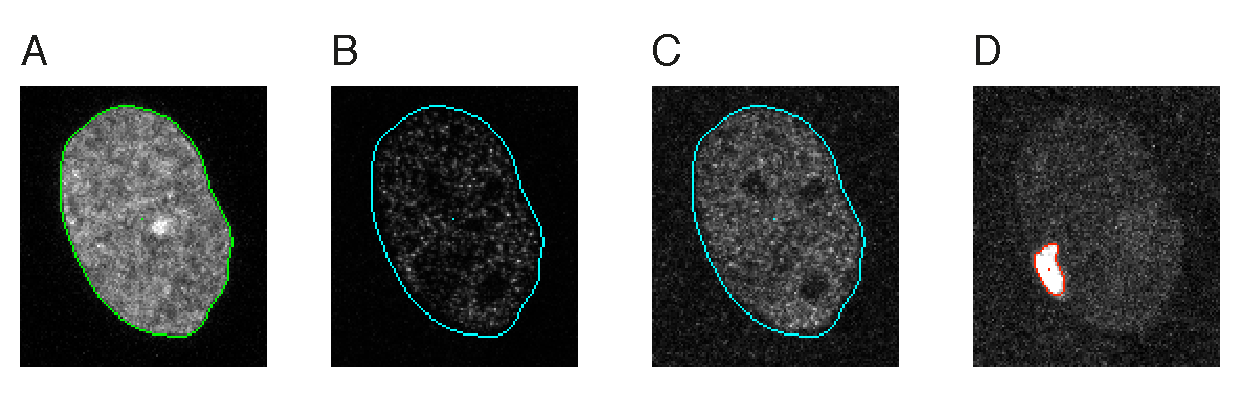
\includegraphics[width=1\textwidth]{Abbildungen/figure4_1.pdf}
		\caption{\textbf{Blubb.} A) B) }
		\label{fig:coStaining}
	\end{center}
\end{figure}

\subsection{Nuclear expression of NER factors is strongly correlated}

\begin{figure}[htbp]
	\begin{center}
		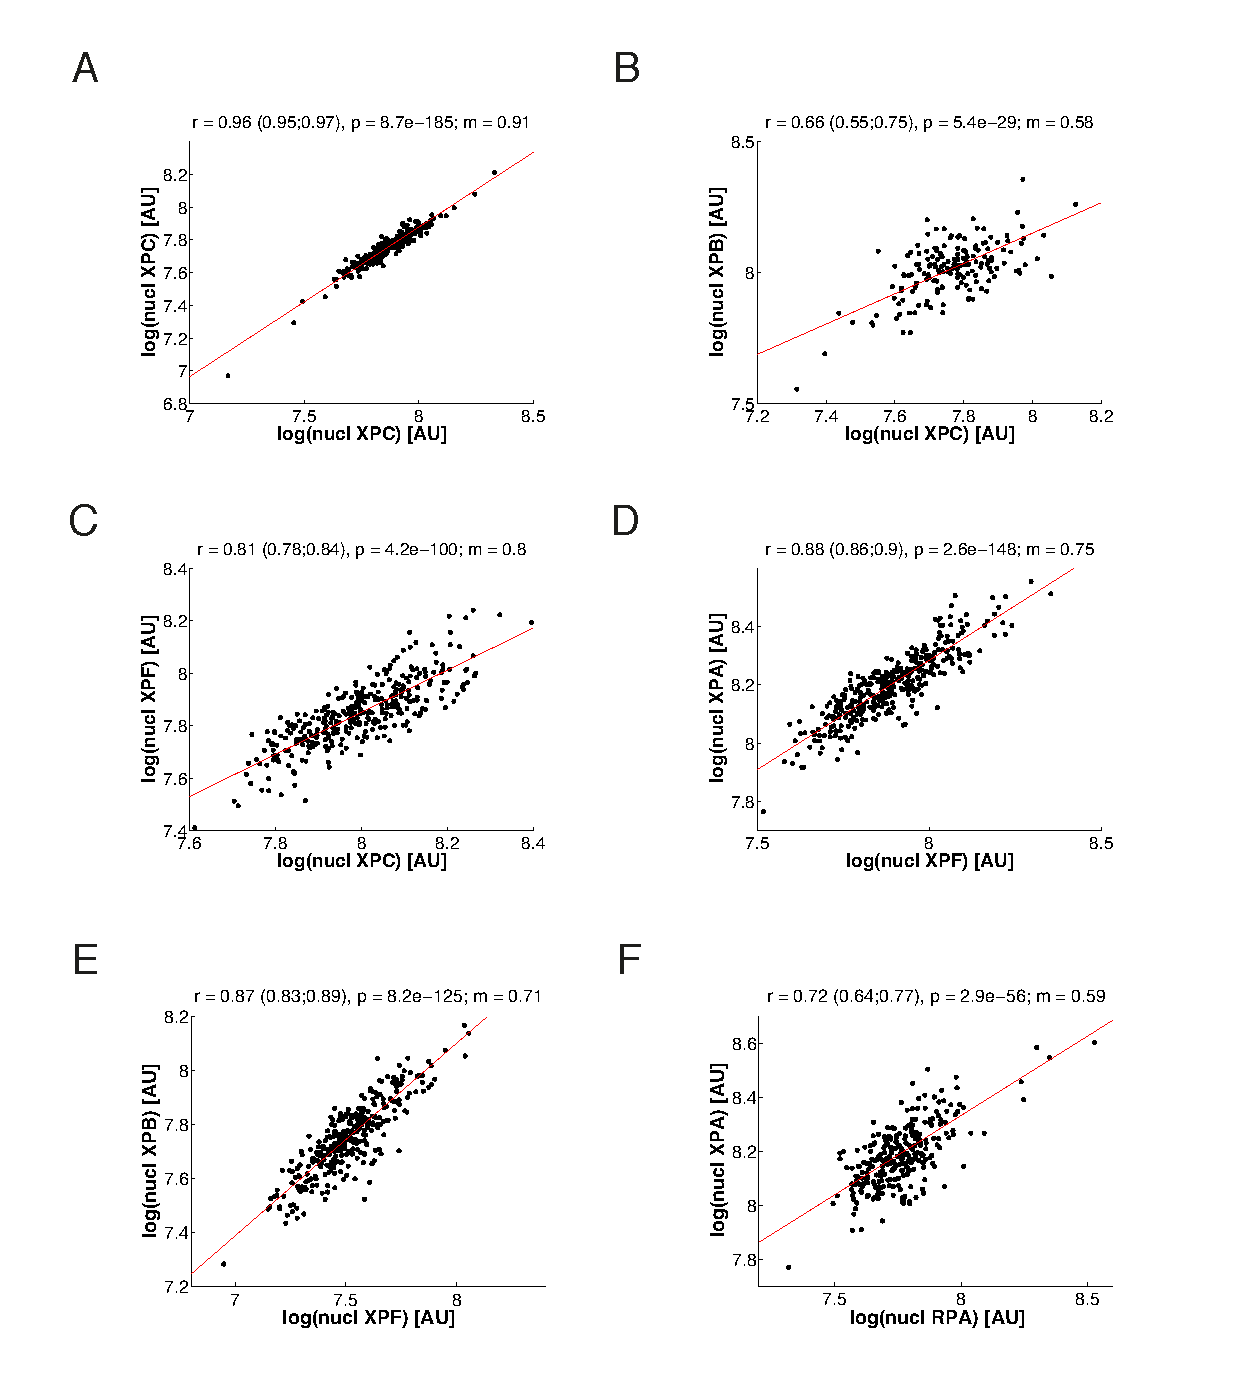
\includegraphics[width=1\textwidth]{Abbildungen/figure4_2.pdf}
		\caption{\textbf{Blubb.} A) B) }
		\label{fig:coExpressionData}
	\end{center}
\end{figure}


\begin{figure}[htbp]
	\begin{center}
		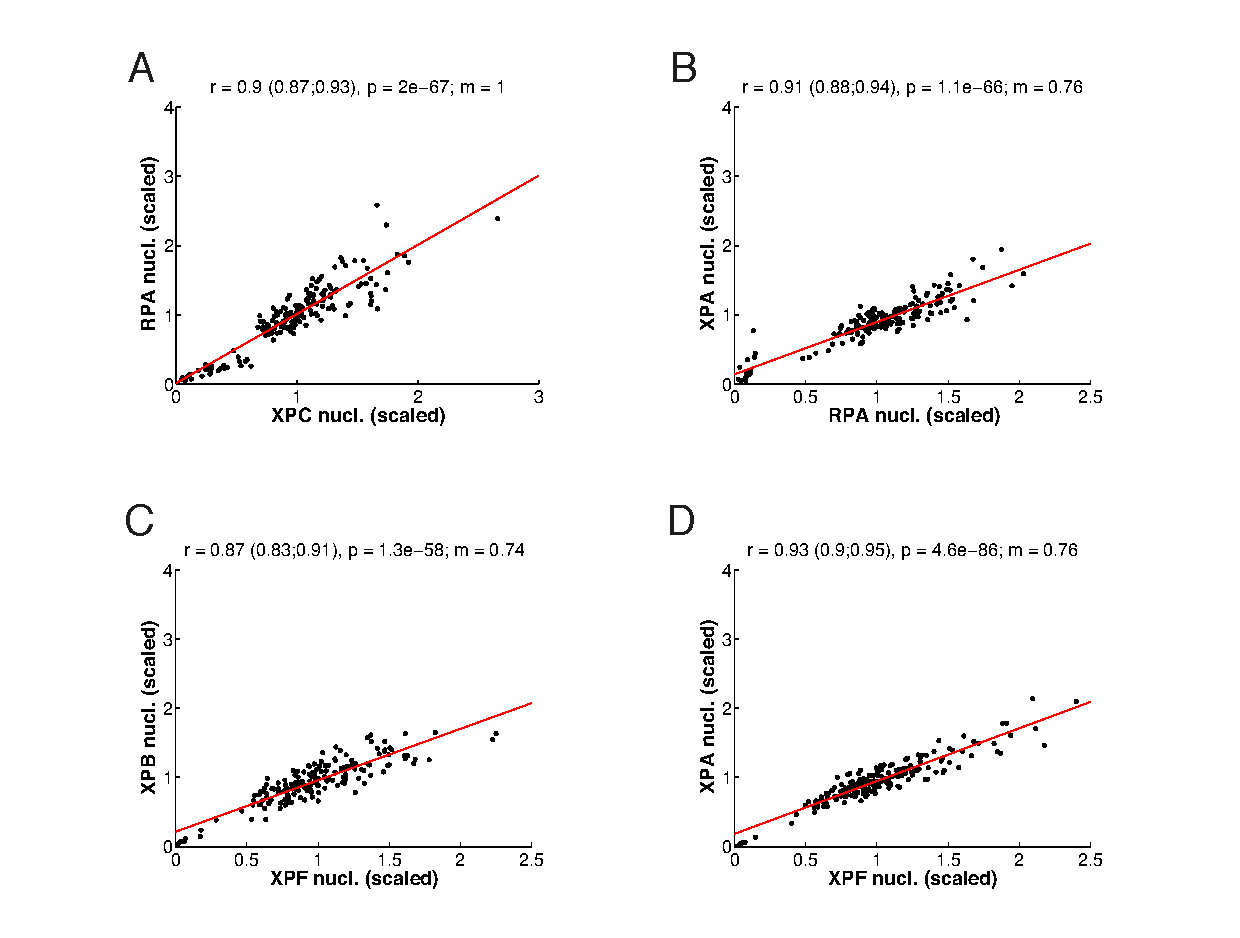
\includegraphics[width=1\textwidth]{Abbildungen/figure4_3.pdf}
		\caption{\textbf{Blubb.} A) B) }
		\label{fig:coExpressionData_woDamage}
	\end{center}
\end{figure}

\subsection{Flow cytometry verification}

